Dans leur article, Hermary et al. \cite{Hermary_2022}, pour tenter de donner une explication aux différents échecs de convergence de leurs expériences, émettaient l'hypothèse que le fait qu'un élément (ou fonction) structurant << touche >> le bord de son support (i.e. le fait qu'il existe un pixel au bord du support de valeur strictement supérieure à 0 pouvant être associée à l'objet de l'image) aide le réseau, lors de son entraînement, à converger de manière plus précise et certaine vers l'élément structurant cible. \\

\vspace{-1.6mm}
\noindent En reproduisant les différentes expériences de leur article, avec notamment leurs six fonctions structurantes cibles telles que décrites dans les grandes parties précédentes (\textit{cross3}, \textit{cross7}, \textit{disk2}, \textit{disk3}, \textit{diamond3} et \textit{complex}), on peut effectivement constater que les cas d'échec interviennent uniquement sur les structures dont aucune partie ne touche le bord de leur support (\textit{cross3} et \textit{disk2}), là où les structures touchant le bord de leur support donnent systématiquement lieu à un succès de convergence (\textit{cross7}, \textit{disk3}, \textit{diamond3} et \textit{complex}), du moins pour ces fonctions structurantes-là (fig. \ref{fig:art_resultats_opening} et \ref{fig:art_resultats_closing}). \\

\vspace{-1.6mm}
\noindent Une explication donnée est le fait que, lors de la rétropropagation du grandient pendant l'apprentissage du réseau, ce sont les poids des bords du support des noyaux $w$ qui semblent se mettre à jour en premier, ou du moins qui convergent plus rapidement. Par exemple, sur la figure \ref{fig:c_awayOPP} montrant l'évolution des deux noyaux du réseau pour la fonction structurante cible \textit{adiag}, avec ou sans contrainte $C_\text{awayOPP}$, on voit lors des premières époques que ce sont effectivement les poids au bord du support qui semblent converger en premier vers leur état final : les coins supérieur gauche et inférieur droit, par lesquels passe la diagonale, prennent en premier les plus grandes valeurs, et les coins supérieur droit et inférieur gauche prennent de plus petites valeurs, là où le centre du support reste creux et surtout très homogène. La forme de la structure semble se dessiner en partant des bords jusqu'au centre du support. \\

\vspace{-1.0mm}
Cependant, avec les deux autres fonctions structurantes créées en plus (\textit{adiag} et \textit{brand}), on remarque que cette propriété n'est ici pas respectée : malgré le fait que \textit{adiag} touche largement les bords d'une part et d'autre de son support, les réseaux $\mathcal{S}$MorphNet et $\mathcal{S}$MorphNetTanh, sans contrainte, ont tous deux du mal à converger vers cette forme diagonale, pour laquelle les métriques de performances des réseaux sont moyennes voire mauvaises (de l'ordre de $10^-3$ pour la \textit{loss}). À l'inverse, pour la fonction structurante \textit{brand}, les deux réseaux arrivent très bien à trouver la forme de la structure cible, malgré le fait que cette dernière ne touche pas le bord (fig. \ref{fig:SMvsSMTH_opening_mnist} et \ref{fig:SMvsSMTH_closing_mnist}). \\

\vspace{-1.6mm}
\noindent Des expériences complémentaires ont été réalisées en ajoutant, dans \textit{brand}, un unique pixel au bord du support. Et les résultats de convergence des réseaux avec cette structure cible-là, qui touche donc le bord, sont même légèrement moins bons que ceux avec la structure \textit{brand} originelle, comme le montre la figure \ref{fig:touch_notouch_borders} ci-après.


\newpage

%figure
%\vspace{-0.8mm}
\begin{figure}[htp]
  \begin{center}
    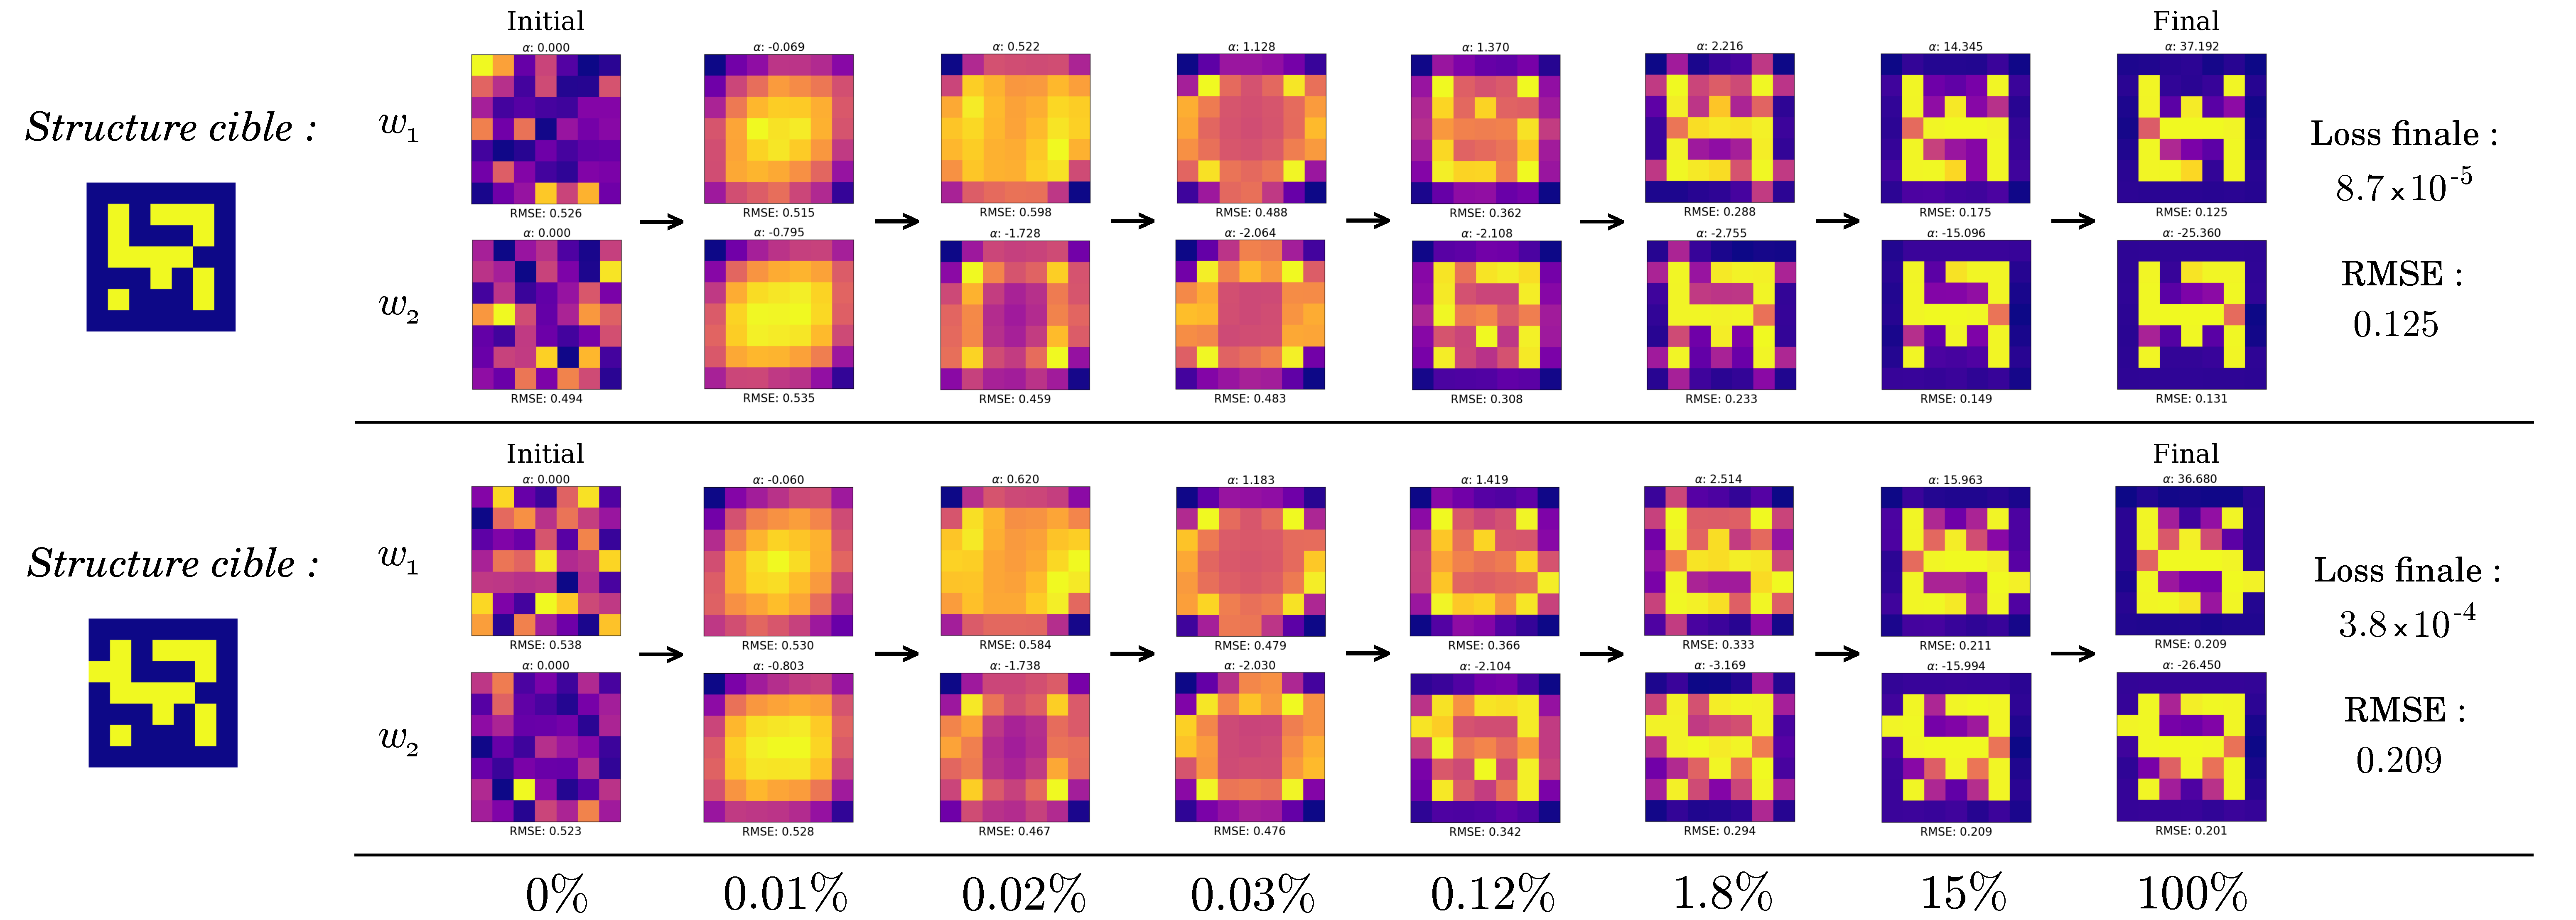
\includegraphics[width=1.00\linewidth]{parts/4-analyse_des_reseaux/complexity_and_fails/figures/z_touchnotouch.pdf}
    \vspace{-4.0mm}
    \caption{ \centering Évolution de la forme des deux noyaux du réseau et de leur \textit{RMSE} en fonction de la progression de l'entraînement (en \% avant l'état final), pour la fermeture sur MNIST, avec le \textit{brand} (haut) et le \textit{brand} avec un pixel en plus au bord (bas).}
    \label{fig:touch_notouch_borders}
  \end{center}
\end{figure}

\vspace{-3.0mm}
L'hypothèse que la structure cible touche (resp. ne touche pas) le bord de son support puisse déterminer le succès (resp. l'échec) de convergence du réseau ne peut donc pas, à elle seule, expliquer l'ensemble des échecs de convergence. En revanche, en exploitant les résultats de convergence de diverses expériences, avec davantage de formes différentes de fonctions structurantes cibles, il semble se dessiner un lien - une correlation positive - entre une certaine << complexité >> de la forme de la structure cible et la réussite du réseau dans sa convergence. En effet, plus la forme de la structure cible semble << complexe >>, plus le réseau semble converger de manière précise et juste, avec des noyaux $w$ de forme davantage proche de celle de la structure cible. \\

\vspace{-2.0mm}
\noindent Cette notion de << complexité >> des fonctions structurantes cibles reste très subjective et mal définie. Elle prend en compte à la fois la \textit{taille} de la structure par rapport à son support (si elle est plus petite, alors les configurations à deux couches où elle est symétriquement translatée sont strictement équivalentes), la multiplicité des \textit{nuances de gris} dont l'élément est composé, et les \textit{caractéristiques topologiques} de cette structure (rotondité, connexité, convexité, extrémités...). Ce premier aspect (élément plus petit que le support) peut expliquer les échecs des cas où l'élément <<ne touche pas le bord>>. \\
%blablabla + impact de la taille du support : plus de variables ! Donc plus de configurations possibles, et plus de minima locaux dans la \textit{loss} \\

\vspace{-2.0mm}
\noindent Cette notion de << complexité >> d'une structure morphologique serait inversement correlée au nombre de décompositions exactes possibles de cet élément dans le cadre d'une érosion ou d'une dilatation. Par exemple, le carré 3x3 peut être considéré comme << peu complexe >>, car il existe une multitude de décompositions de cette structure, par exemple celle en deux segments successifs de longeur 3 (et de largeur 1), l'un horizontal et l'autre vertical, dans le cadre d'une érosion ou d'une dilatation. C'est une explication fort probable des nombreux échecs de convergence des réseaux à deux couches avec comme structure cible le carré 3x3 sur un support de taille 7x7 (en plus de la taille du support qui multiplie les configurations possibles).


\newpage

Une explication possible à cette correlation positive entre complexité de la forme de la structure cible et succès de convergence des réseaux, est le fait que plus la structure est complexe, plus elle est << unique >> : il existerait moins de formes différentes possibles << proches >> morphologiquement parlant de cette structure, et moins de décompositions possibles de cet élément en plusieurs sous-éléments distincts (dans le cadre de réseaux multi-couches). Cette diminution du nombre de formes théoriques possibles << proches >> de la structure visée équivaut à une diminution du nombre de minima locaux possibles dans la fonction de perte \textit{loss} qui sont << proches >> du minimum global associé à la structure cible. Ce qui ferait ainsi que les noyaux $w$ du réseau arrivent mieux à converger vers cette structure cible, et avec plus de précision et de rapidité, car il y aurait moins de minima locaux proches de ce minimum global visé. À l'inverse, une structure cible trop << élémentaire >> impliquerait une multiplicité des solutions locales possibles (i.e. minima locaux dans la \textit{loss}), et donc amènerait davantage le réseau à converger vers l'un de ces minima locaux (un mauvais résultat). \\

\vspace{-1.6mm}
\noindent Ces explications restent néanmoins au stade d'hypothèses, qui doivent être vérifiées et validées. La notion de << complexité >> d'une forme reste également très subjective, et une définition précise de ce terme doit être formulée. Son rôle dans les succès ou les échecs de convergence des réseaux pourrait alors être évalué et quantifié.


\vspace{1.0mm}


%Parler de la relation entre "complexité de la forme du noyau" et multiplicité des solutions locales possibles (minima locaux dans la loss) et mauvaise convergence des réseaux... 
%+ Parler de la définition très vague de la notion de "complexité" des formes : comment savoir si une forme est plus << complexe >> qu'une autre ? Réponse proposée : le nombre de décompositions possibles de cet élément dans le cadre d'une érosion ou dilatation. \\

%%%-> Parler de l'impact de la complexité de la forme des noyaux ("complexité" + parler de si il touche le bord ou non [7], qui n'est pas non plus une hypothèse qui suffit seule à elle-même car il y a des cas où si l'élément structurant touche le bord en ajoutant un seul pixel, alors la convergence est moins bonne que sans ce dernier pixel)! Prendre l'exemple du carré 3x3... (+ impact de la taille du support : plus de variables ! Donc plus de configurations possibles, et plus de minima locaux dans la \textit{loss})